\subsubsection{Project Binder}\label{seq:project-binder}

The Binder Project \cite{binder} (\url{https://jupyter.org/binder}) is
a subproject of the Jupyter project. The Binder project is formally operating
within the Jupyter ecosystem, but not confined to be useful for notebooks.

The key components of the Binder software are \repotodocker{}
(Section~\ref{sec:repo2docker}) and \binderhub{}. The \repotodocker{} tool
creates a software environment inside a Docker container from a software
specification in a repository. \binderhub{} starts a Jupyter notebook server
within this container from which the user can execute the notebooks from the
repository.

\emph{MyBinder} (see \ref{sec:mybinder}) is a service run by the \emph{BinderHub
  federation}\footnote{\url{https://mybinder.readthedocs.io/en/latest/about/federation.html}}
of organisations that collectively host a service running the Binder software
under the URL \url{https://mybinder.org}. This is the service we made use of in
our example in section~\ref{sec:reproducibility-example}.

The focus for this proposal is to improve \repotodocker{}. In particular,
\repotodocker{} solves software environment challenge (see
Section~\ref{sec:reproducibility-concept}) in generic way and is independent
from Jupyter notebooks.

\TODO{Add image that depicts this Jupyter/Binder relation ship}.

\paragraph{Basic functionality of Binder}
\label{binder-how-does-it-work}

The most common reproducibility use case -- with the current state of the Binder
tools -- is the one we introduced in
Section~\ref{sec:terminology}. We will use this to
describe the role of the individual components of Binder:

\begin{figure}
  \centering
  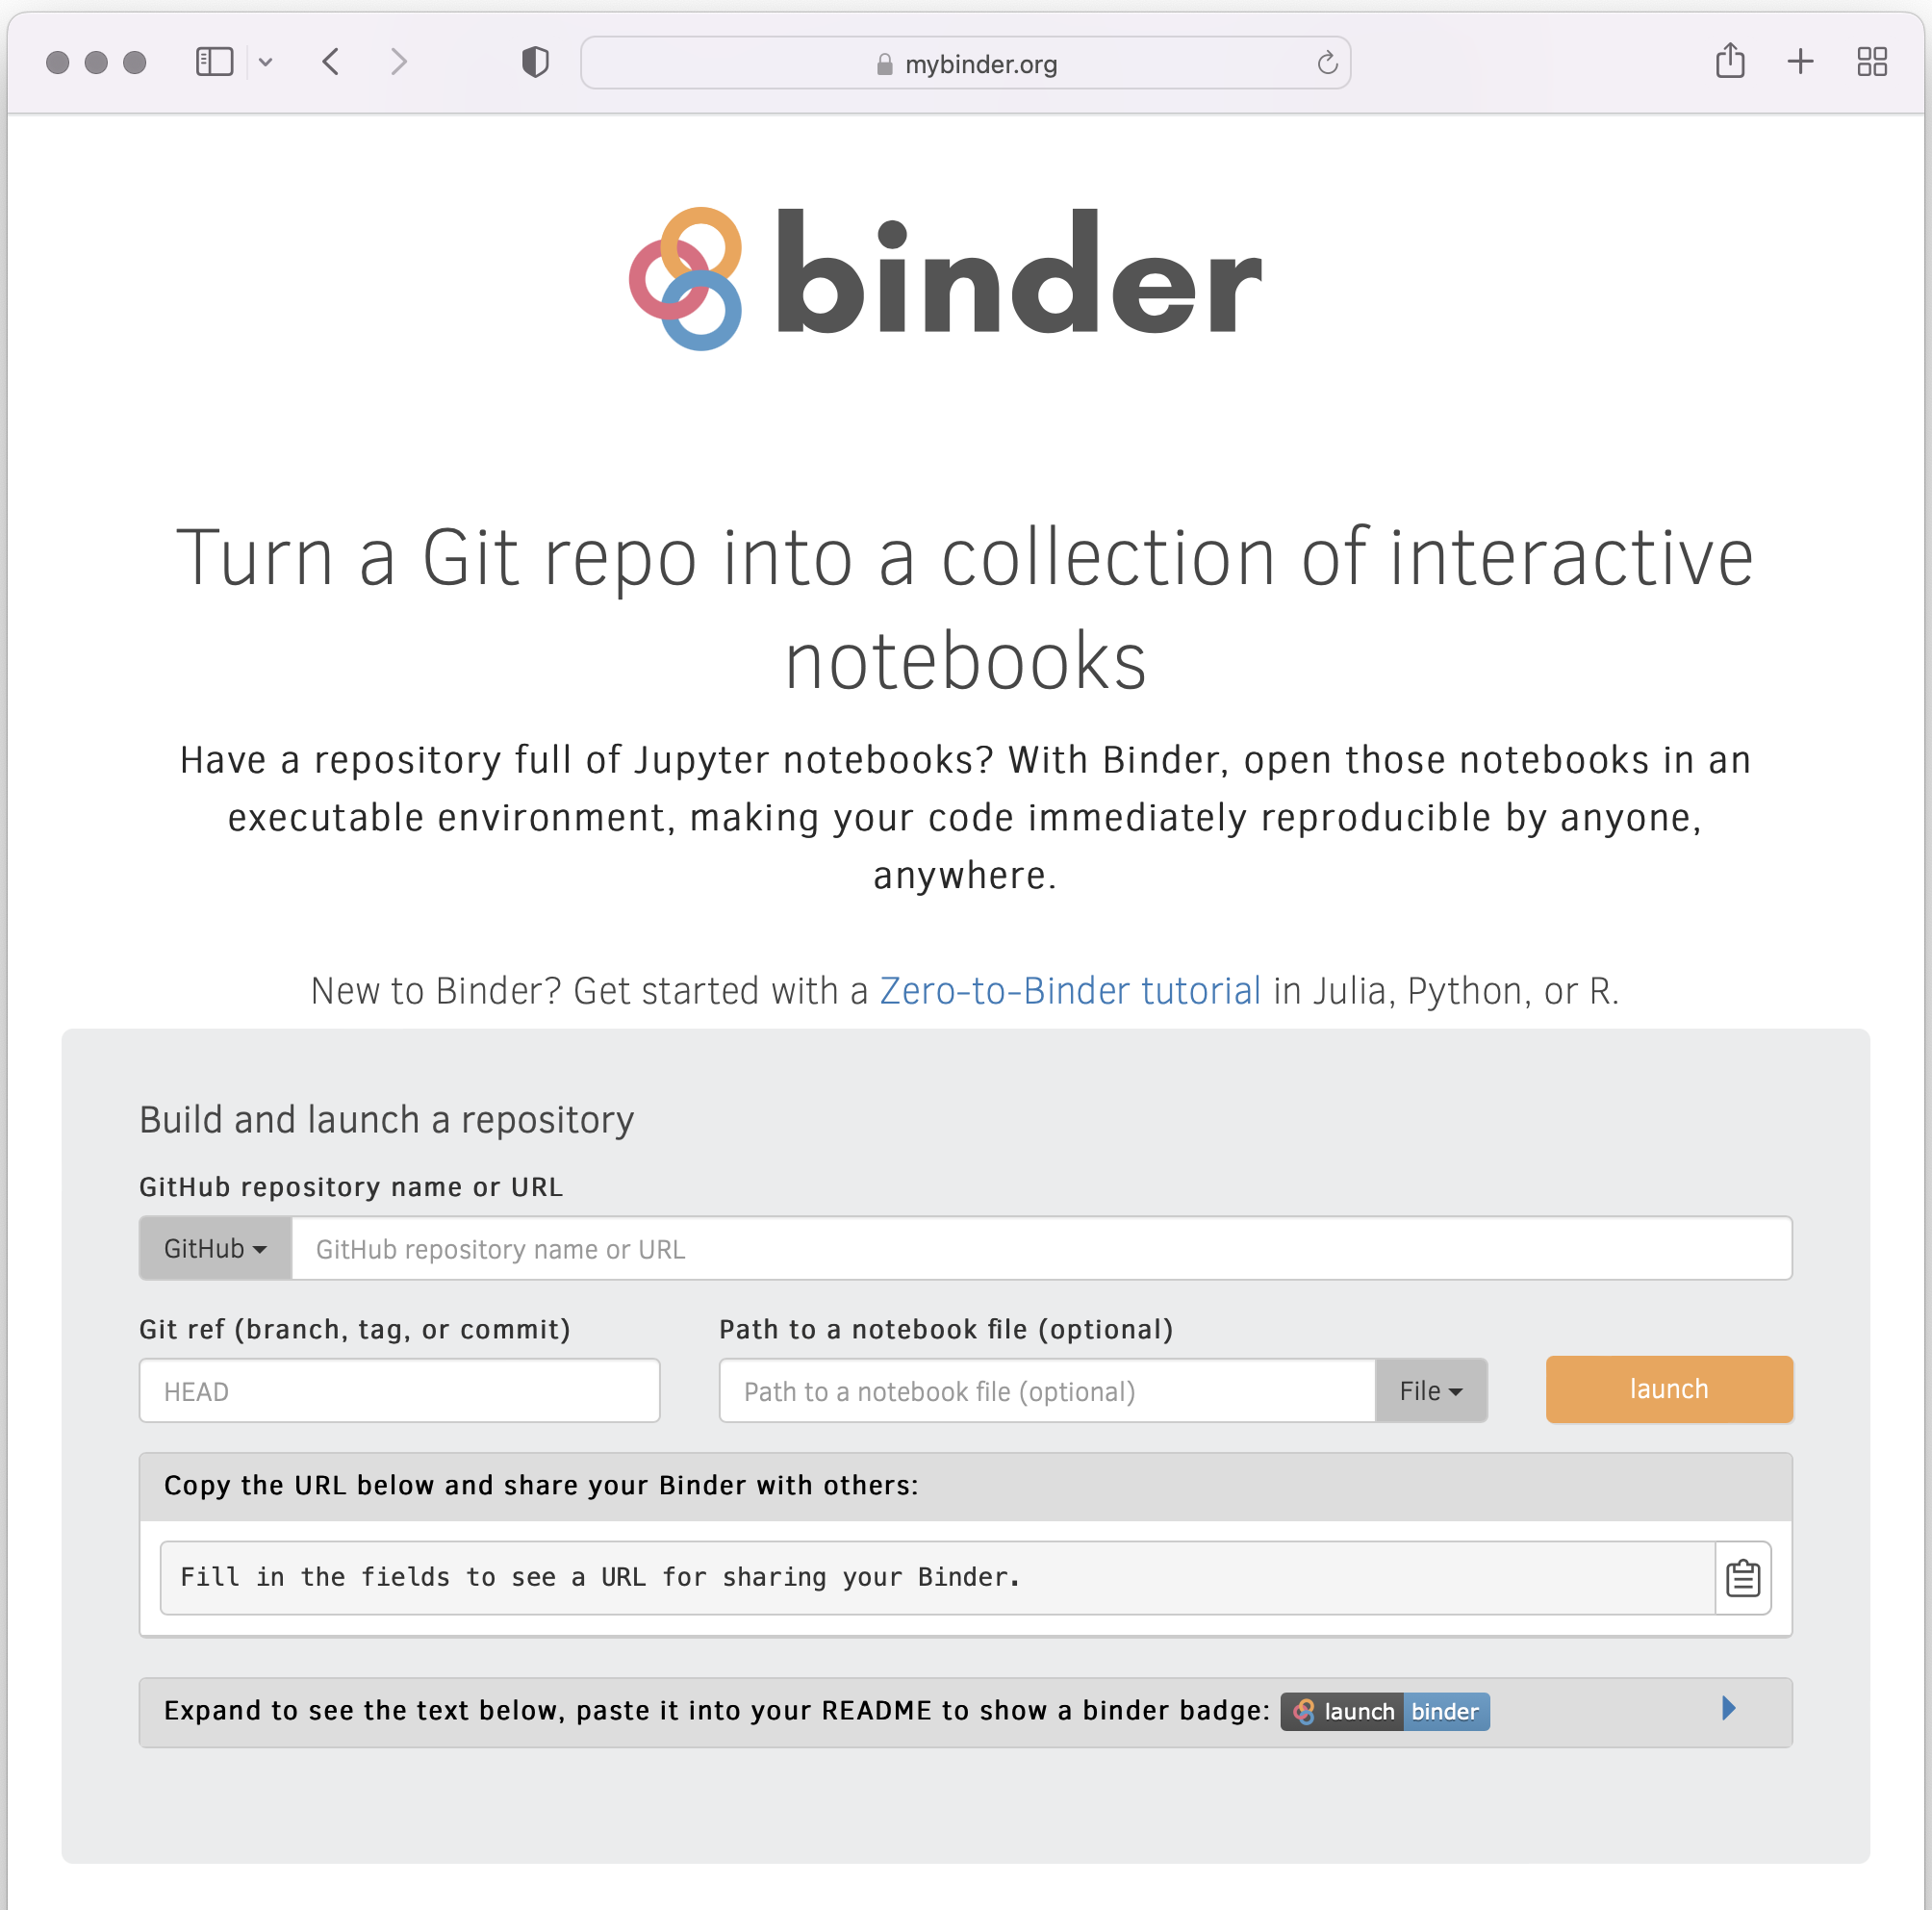
\includegraphics[width=0.7\textwidth]{images/mybinder.png}
  \caption{Home page of the mybinder service.}
  \label{fig:mybinder-homepage}
\end{figure}

\begin{compactitem}
\item The mybinder service is called with a URL that encodes the location of the data
  repository\footnote{For example
    {\url{https://mybinder.org/v2/gh/fangohr/reproducibility-repository-example/HEAD?labpath=figure1.ipynb}}
    referring to the GitHub repository REPRODUCIBILITY-REPOSITORY-EXAMPLE of the
    github user FANGOHR, asking to open FIGURE1.IPYNB file.}

  Alternatively, there is form (see Figure~\ref{fig:mybinder-homepage})
  which users can complete with repository details
  to start the build of the corresponding environment, or to obtain the URL to
  re-use that configuration later, or share it with others.
\item From the mybinder.org entry point, the request is forwarded to one
  \binderhub{} service of one of the organisations in the BinderHub federation
  that has available compute capacities.
\item The \binderhub{} software running at the chosen location, will ask
  \repotodocker{} to create a docker container in which the notebooks from the repository can be executed.
\item \repotodocker{} searches the repository for specifications of software requirements (see \ref{repo2docker-supported-software-specifications}).
\item \repotodocker{} composes a Dockerfile that contains all the commands
  necessary to install software.
\item \repotodocker{} builds the Docker image based on the Dockerfile
\item \binderhub{} takes the Docker image and asks Kubernetes to start up
  container based on this image
\item The notebook server is started in this Docker container.
\item \binderhub{} forwards the user who requested this virtual environment to
  the URL at which the repository (or a particular notebook) can be explored
  from within the Jupyter notebook (which runs in the container).
\end{compactitem}

\paragraph{\repotodocker}\label{sec:repo2docker}
\TODO{Hans: I think we refer to this section from various places, but we have
  introduced the role of repo2docker already above in
  \ref{binder-how-does-it-work}. What should/could we add here?}

\paragraph{Supported software specification formats}
\label{repo2docker-supported-software-specifications}
The \repotodocker{} tool currently supports the following software specification
formats to build Docker images:
% source:
% https://repo2docker.readthedocs.io/en/latest/config_files.html#config-files
% 9 April 2022
\begin{compactitem}
\item \softwarename{requirements.txt}, \softwarename{setup.py},
  \softwarename{Pipfile}, \softwarename{Pipfile.lock}: to specify Python
  packages and environments
\item \softwarename{Project.toml}, \softwarename{JuliaProject.toml} and (legacy)
  \softwarename{REQUIRE}: to
  specify Julia version and packages
\item \softwarename{install.R}, \softwarename{DESCRIPTION}: to install R
  libraries, or install the repository as R package
\item \softwarename{apt.get}: to install Debian packages. The Docker container
  is currently based on Ubuntu, which uses the Debian package management tool \softwarename{apt}.
\item \softwarename{environment.yml}: to specify conda packages and
  environments
\item \softwarename{default.nix}: to use the nix package manager for software provision
\item \softwarename{Dockerfile}: providing a Dockerfile enables users to define
  virtually arbitrary environments, for example based on software from the
  repositories of Linux distributions.
\end{compactitem}

\medskip
\subsubsection{Binder for reproducibility}\label{sec:binder-for-reproducibility}
\TOWRITE{}{}


\subsubsection{Related project: Mybinder}\label{sec:mybinder}

\TOWRITE{}{The MyBinder.org federation}


%%% Local Variables:
%%% mode: latex
%%% TeX-master: "proposal"
%%% End:
